% =========================================================================
%  VisionCart -- Project Manual
%  Generated from a full inspection of the running application and source.
%  Compile with:  pdflatex MANUAL.tex   (run twice for the table of contents)
% =========================================================================
\documentclass[11pt,a4paper]{report}

\usepackage[utf8]{inputenc}
\usepackage[T1]{fontenc}
\usepackage{lmodern}
\usepackage[margin=2.4cm]{geometry}
\usepackage[dvipsnames,table]{xcolor}
\usepackage{booktabs}
\usepackage{longtable}
\usepackage{array}
\usepackage{amsmath}
\usepackage{amssymb}
\usepackage{enumitem}
\usepackage{fancyhdr}
\usepackage{titlesec}
\usepackage{tikz}
\usepackage{listings}
\usepackage{caption}
\usepackage{float}
\usepackage[hidelinks,bookmarks=true]{hyperref}

\usetikzlibrary{shapes.geometric,arrows.meta,positioning,fit,backgrounds,calc}

% ---------------------------------------------------------------- colours --
\definecolor{vcblue}{HTML}{0B5FA5}
\definecolor{vcink}{HTML}{1A2230}
\definecolor{vcgrey}{HTML}{5B6472}
\definecolor{vclight}{HTML}{F1F4F8}
\definecolor{vcgreen}{HTML}{1B7A47}
\definecolor{vcamber}{HTML}{9A6B08}
\definecolor{vcred}{HTML}{A32828}

% ---------------------------------------------------------------- styling --
\titleformat{\chapter}[display]
  {\normalfont\huge\bfseries\color{vcblue}}
  {\normalsize\color{vcgrey}\MakeUppercase{\chaptertitlename}\ \thechapter}
  {8pt}{\Huge}
\titlespacing*{\chapter}{0pt}{-18pt}{22pt}

\titleformat{\section}{\normalfont\Large\bfseries\color{vcink}}{\thesection}{0.7em}{}
\titleformat{\subsection}{\normalfont\large\bfseries\color{vcgrey}}{\thesubsection}{0.7em}{}

\pagestyle{fancy}
\fancyhf{}
\fancyhead[L]{\small\color{vcgrey}VisionCart --- Project Manual}
\fancyhead[R]{\small\color{vcgrey}\thepage}
\renewcommand{\headrulewidth}{0.4pt}

\setlist[itemize]{leftmargin=1.4em,itemsep=2pt,topsep=3pt}
\setlist[enumerate]{leftmargin=1.6em,itemsep=2pt,topsep=3pt}

\lstset{
  basicstyle=\ttfamily\footnotesize,
  backgroundcolor=\color{vclight},
  frame=single,
  rulecolor=\color{vcgrey!40},
  breaklines=true,
  showstringspaces=false,
  columns=fullflexible,
  xleftmargin=4pt,
  framexleftmargin=4pt
}

% ----------------------------------------------------------------- macros --
\newcommand{\code}[1]{\texttt{\small #1}}
\newcommand{\built}{\textcolor{vcgreen}{\textbf{Built}}}
\newcommand{\partly}{\textcolor{vcamber}{\textbf{Partial}}}
\newcommand{\absent}{\textcolor{vcred}{\textbf{Missing}}}

\newcommand{\keybox}[2]{%
  \begin{center}
  \begin{minipage}{0.94\textwidth}
  \colorbox{vclight}{\parbox{\dimexpr\textwidth-2\fboxsep}{%
    \vspace{3pt}\textbf{\color{vcblue}#1}\\[3pt]#2\vspace{4pt}}}
  \end{minipage}
  \end{center}}

% ------------------------------------------------------------------ title --
\begin{document}
\begin{titlepage}
\centering
\vspace*{2.2cm}
{\color{vcgrey}\Large A COMPLETE PROJECT MANUAL}\\[1.1cm]
{\color{vcblue}\Huge\bfseries VisionCart}\\[0.45cm]
{\Large\bfseries A prescription eyewear shop with virtual try-on}\\[1.4cm]
\rule{0.75\textwidth}{0.9pt}\\[0.8cm]
\begin{minipage}{0.78\textwidth}
\centering\large
What the project is, how much of it is finished, what is still\\
missing, which technologies it uses, and how it is put together.\\[0.6cm]
\normalsize\color{vcgrey}
Written for a reader with no programming background,\\
with full technical detail in the later parts.
\end{minipage}\\[1.6cm]
\rule{0.75\textwidth}{0.9pt}\\[1.0cm]
{\color{vcgrey}\normalsize
Version 0.1.0 \quad$\cdot$\quad Assessed 24 August 2026\\[3pt]
Based on inspection of the running application and all 77 source files}
\vfill
\end{titlepage}

\tableofcontents
\newpage

% =========================================================================
\part{The project in plain language}
% =========================================================================

\chapter{What this project is}

\section{The one-sentence version}

\keybox{In one sentence}{VisionCart is a complete website for an
opticians' shop: customers can see how a pair of glasses looks on their own
face before buying, enter their eye prescription, and order lenses made to
it --- while the shop's staff run the entire business, from stock to patient
records to the lens lab, from a private back-office area of the same site.}

\section{The problem it solves}

Buying spectacles online has always been awkward for two reasons.

\begin{enumerate}
  \item \textbf{You cannot see how they look on you.} A photograph of a
        frame on a white background tells you almost nothing about whether it
        suits your face or fits your head.
  \item \textbf{Spectacles are a medical product.} They are made to a
        prescription written by an eye specialist. Get one number wrong and
        the customer gets a headache, and the shop pays to have the lenses cut
        again. A normal online shop --- the kind that sells shoes --- has no
        idea what any of that means.
\end{enumerate}

VisionCart answers both. It puts a \textbf{virtual mirror} on the website that
places the frame on the customer's own photograph at the correct size, and it
treats every customer as a \textbf{patient with a file}, the way a real
opticians' practice does.

\section{The two halves of the product}

The software is really two applications sharing one database.

\begin{center}
\begin{tabular}{@{}p{0.45\textwidth}p{0.45\textwidth}@{}}
\toprule
\textbf{The shop (public)} & \textbf{The back office (staff only)}\\
\midrule
What a customer sees. Browse frames, try them on, choose lenses, enter a
prescription, pay, and track the order.
&
What the shop's own people see. Stock, photographs, patient files,
prescriptions, orders, the lens lab queue, discounts, and settings.\\
\addlinespace
13 pages & 16 pages\\
Anyone can visit & Requires a staff login\\
\bottomrule
\end{tabular}
\end{center}

\section{Who it is for}

\begin{itemize}
  \item \textbf{The customer} --- anyone who needs glasses and would rather
        not spend an afternoon in a shop.
  \item \textbf{Shop staff} --- take orders, manage stock, upload product
        photographs, chase the lab.
  \item \textbf{The optician} --- the qualified person who checks that every
        prescription a customer typed in is sensible before lenses are cut.
  \item \textbf{The owner or administrator} --- prices, discounts, staff
        accounts, and the shop's rules.
\end{itemize}

\chapter{How it works, step by step}

\section{A customer's journey}

\begin{enumerate}
  \item \textbf{Browsing.} The customer opens the shop and sees the frames.
        They can narrow the list by who it is for, the shape, the material,
        the brand, the size, or the price.

  \item \textbf{The virtual mirror.} They upload a photograph of their face,
        or switch on their camera. The website finds their eyes and places the
        chosen frame over the photograph at the right size and angle. They can
        flick through every frame in the shop and watch each one land on their
        face.

  \item \textbf{The measurement.} While it is doing that, the website
        measures the distance between the customer's pupils --- an essential
        number for making lenses, which most people do not know. It is honest
        about the accuracy and always says an optician will confirm it.

  \item \textbf{Choosing lenses.} The customer walks through six questions:
        what the glasses are for, the lens type, the thickness, the coatings,
        the tint, and any extras. Each answer shows what it adds to the price.
        The shop currently offers 24 different lens choices.

  \item \textbf{The prescription.} They either type it in --- using drop-down
        menus only, never a free-text box --- or upload a photograph of the
        paper prescription for the optician to read.

  \item \textbf{Paying.} They fill in a delivery address, pick a delivery
        speed and a payment method, and place the order. They do not need an
        account.

  \item \textbf{Afterwards.} They get an order page they can return to. If
        they made an account, their prescription is stored and can be reused
        next time.
\end{enumerate}

\section{A day in the back office}

\begin{enumerate}
  \item The \textbf{dashboard} opens on the numbers that matter today:
        orders taken, money received, prescriptions waiting to be checked,
        and which frames are running low.

  \item The \textbf{optician} works through the prescription queue. Each one
        is either verified or rejected. Nothing goes to the lens lab until a
        qualified person has approved it.

  \item Staff open each \textbf{order}. Every order line carries its own
        \emph{lab ticket}: the exact prescription, the lens choices, and a
        stage marker that moves from \emph{pending} through \emph{surfacing},
        \emph{coating} and \emph{glazing} to \emph{ready}.

  \item Payment is confirmed, a courier and tracking number recorded, and the
        order is marked shipped.

  \item In quieter moments: new frames are added, a photography shoot is
        dragged into the media library, prices are adjusted, and discounts are
        created --- all of which take effect on the shop immediately.
\end{enumerate}

\section{Why the prescription rules are so strict}

\keybox{The most important design decision in the whole project}{Every
prescription number is chosen from a drop-down list, never typed. Eye
prescriptions move in steps of 0.25 --- $-2.00$, $-2.25$, $-2.50$ and so on.
If a customer could type freely, someone would eventually enter $-2.13$, which
no lens laboratory can make. The order would be accepted, the lenses cut wrong,
and the shop would pay to remake them. Removing the text box removes the whole
class of error.}

Three further rules follow from the same thinking:

\begin{itemize}
  \item A prescription is \textbf{never edited once it has been used}. A new
        version is created instead, so an invoice from three years ago still
        reads correctly.
  \item Each order line keeps its \textbf{own frozen copy} of the
        prescription, independent of the patient's file.
  \item A ``cylinder'' value without an ``axis'' value, or the reverse, is
        \textbf{rejected}, because one is meaningless without the other.
\end{itemize}

\section{What happens to the customer's photograph}

This is worth stating plainly because it is unusual.

\keybox{Photographs stay on the customer's own computer}{The face-detection
software runs \emph{inside the customer's web browser}. The photograph and the
camera feed never travel to the shop's server. The only image that can ever
reach the server is the finished picture the customer explicitly presses
``save'' on --- and even that is switched \textbf{off} by default. With it off,
the server refuses such uploads outright rather than merely hiding the button.
Customers can still download their own picture either way.}

% =========================================================================
\part{How much is finished, and what is not}
% =========================================================================

\chapter{How this assessment was made}

The figures in this part are not taken from the project's own documentation.
They come from three checks carried out directly on this copy of the project:

\begin{enumerate}
  \item \textbf{The application was started and used.} The development server
        was launched and every public page and every back-office page was
        opened in a real browser and exercised.
  \item \textbf{Every source file was read.} All 77 TypeScript files, the
        database schema, the seed data and the two asset scripts.
  \item \textbf{The automated checks were run.} The TypeScript compiler and
        the code linter were both run over the whole project.
\end{enumerate}

\keybox{Headline result}{The project builds cleanly, runs, and does what it
claims to do. The type checker reports \textbf{zero errors} and the linter
reports \textbf{zero warnings}. Everything the shop needs in order to take an
order and fulfil it is present and working. What is missing is the ring of
supporting machinery a live business needs around that core --- chiefly email,
password recovery, abuse protection, and automated tests.}

\chapter{What is finished and verified working}

\section{Verified in a live browser session}

Each item below was opened and used in the running application, not merely
read in the source code.

\begin{longtable}{@{}p{0.28\textwidth}p{0.63\textwidth}@{}}
\toprule
\textbf{Area} & \textbf{What was confirmed}\\
\midrule
\endfirsthead
\toprule
\textbf{Area} & \textbf{What was confirmed}\\
\midrule
\endhead
Home page & Renders with a live promotional banner, a three-step explainer,
and a ``popular this season'' grid drawn from the database.\\
\addlinespace
Frame catalogue & 10 frames in 30 colour variants, all with generated
artwork. Filters for search, wearer, shape, rim, brand, collection, size and
sort all render. Sale badges and colour swatches correct.\\
\addlinespace
Product page & Full specification table, four colour thumbnails, and the
complete lens builder: 24 options across 6 groups, each showing its price
supplement. Prescription drop-downs present with the full 0.25 range.\\
\addlinespace
Virtual try-on & The studio loads and offers all 30 frames. The face-detection
model initialised successfully in the browser, proving the 3.6\,MB model and
the 34\,MB WebAssembly runtime are served correctly from the project itself
rather than from an outside network.\\
\addlinespace
Shopping bag & A frame was added to the bag successfully. Quantity controls,
removal and the bag summary all work.\\
\addlinespace
Discounts & The code \code{WELCOME15} was applied and correctly reduced a
Rs.\,6{,}500 frame by Rs.\,975, exactly 15\%, producing a Rs.\,5{,}825 total
after Rs.\,300 delivery. The arithmetic is exact, with no rounding drift.\\
\addlinespace
Checkout & Guest checkout renders with contact fields, address, two delivery
speeds priced from the rate table, and two payment methods. The card option
was correctly hidden because no card-processor key is configured.\\
\addlinespace
Access control & Visiting the back office, the customer account area or the
checkout without a session correctly redirects to the sign-in page in every
case tested.\\
\addlinespace
Back office, dashboard & Eight live figures, a prescription queue, recent
orders and a low-stock table, all reading real data.\\
\addlinespace
Back office, orders & Order list with status and payment filters. The order
detail page shows the lab ticket with the frozen prescription, a lab-stage
selector, a full price breakdown, payment controls and courier controls.\\
\addlinespace
Back office, patients & Patient file with contact details, clinical notes,
consent flag, pupil measurements, the full prescription history, and
verify/reject controls. A new prescription can be added from the same screen.\\
\addlinespace
Back office, frames & Complete product editor: identity, style, six
measurements, pricing, selling rules, search listing, plus colourway
management showing stock and try-on calibration status per colour.\\
\addlinespace
Back office, lenses & Every lens option listed by group with its price,
prescription limits, default flag and live flag, each editable.\\
\addlinespace
Back office, promotions & Four seeded deals listed with code, type, value,
date window and usage, each editable.\\
\addlinespace
Back office, media & Drag-and-drop library with batch tagging and search.\\
\addlinespace
Back office, import & Four spreadsheet exports and two imports, with a
documented column reference, a compulsory dry-run check, and a history of past
import jobs including a deliberately broken file that was correctly reported
as ``1 ok, 2 failed''.\\
\addlinespace
Back office, settings & Store details, selling rules and three try-on
switches, plus a read-only panel confirming which integrations are live.\\
\bottomrule
\end{longtable}

\section{Depth of the underlying implementation}

Several parts go considerably further than a demonstration would require.

\begin{itemize}
  \item \textbf{Payments} are genuinely implemented for all three methods, not
        stubbed. Cash on delivery and bank transfer are complete; the card
        route creates a real hosted checkout session, confirms the order from
        the provider's webhook rather than from the customer's browser
        returning, and can issue real refunds.
  \item \textbf{Shipping} has three implementations. The default reads a rate
        table. The two live-carrier options make real calls to their
        providers and can buy a real printable label --- and both fall back to
        the rate table if the key is absent or the call fails.
  \item \textbf{Image storage} works locally with no setup, and has a complete
        cloud implementation that loads its cloud library only when actually
        used. Every upload is rotated from its embedded orientation, capped at
        2000 pixels, converted to a modern format and thumbnailed.
  \item \textbf{Spreadsheet handling} is written from scratch and correctly
        handles quoted fields, embedded commas and line breaks, doubled
        quotes, Windows line endings, and the invisible marker Excel puts at
        the start of a file.
  \item \textbf{Auditing} is wired into 26 places across the codebase. Every
        change to a patient record, a price or an order is recorded with who
        did it and from where.
\end{itemize}

\chapter{What is not built}

\section{Gaps the project itself declares}

The project's own documentation is honest about four omissions. All four were
confirmed by searching the source code.

\begin{longtable}{@{}p{0.22\textwidth}p{0.14\textwidth}p{0.54\textwidth}@{}}
\toprule
\textbf{Gap} & \textbf{Status} & \textbf{What it means in practice}\\
\midrule
\endhead
Order emails & \absent &
The configuration file has a mail setting, but there is not one line of code
anywhere in the project that sends an email. A customer who orders receives no
confirmation. This is the single most important gap.\\
\addlinespace
Password recovery & \absent &
A customer or member of staff who forgets their password cannot recover it.
There is no ``forgotten password'' link and no reset mechanism.\\
\addlinespace
Abuse protection & \absent &
Nothing limits how many times the sign-in form or the file-upload endpoints
can be hit. Passwords could be guessed by brute force, and the upload routes
could be flooded.\\
\addlinespace
Automated tests & \absent &
There are no tests of any kind and no test framework installed. The two most
obviously testable parts, the try-on geometry and the discount engine, are
deliberately written as self-contained mathematics precisely so they can be
tested, but nobody has written the tests.\\
\bottomrule
\end{longtable}

\section{Further gaps found during this inspection}

These are not mentioned in the project's own documentation.

\begin{longtable}{@{}p{0.22\textwidth}p{0.15\textwidth}p{0.53\textwidth}@{}}
\toprule
\textbf{Gap} & \textbf{Severity} & \textbf{Detail}\\
\midrule
\endhead
Four broken links & \textcolor{vcred}{Customer-visible} &
The footer of every public page links to four guide pages: how to read a
prescription, measuring your pupil distance, returns, and privacy. None of the
four exists; all return ``page not found''.\\
\addlinespace
No error pages & \textcolor{vcamber}{Cosmetic} &
The project defines no custom ``not found'' or ``something went wrong''
screens, so those four broken links land on the framework's bare default page
rather than on the shop's own design.\\
\addlinespace
Appointments & \textcolor{vcamber}{Unused} &
The database has a full appointments table --- eye tests, fittings,
collections, adjustments, follow-ups --- and not a single line of code
anywhere reads or writes it. It is a designed-but-unbuilt feature.\\
\addlinespace
No audit viewer & \textcolor{vcamber}{Operational} &
The audit trail is written faithfully in 26 places but there is no screen
anywhere that reads it back. To answer ``who changed this price?'' somebody
must query the database directly.\\
\addlinespace
No delivery-rate editor & \textcolor{vcamber}{Operational} &
Delivery prices live in a database table that only the code reads. The
documentation states these are editable in the back office, but no such screen
exists; the settings page only displays which provider is active. To change a
delivery price today you must edit the database.\\
\addlinespace
No address book & \textcolor{vcgrey}{Minor} &
Addresses are saved at checkout but there is no screen where a customer can
review, edit or delete them afterwards.\\
\addlinespace
Cloud file deletion & \textcolor{vcgrey}{Minor} &
When a picture is deleted and the shop is using cloud storage, the database
record goes but the file itself is deliberately left in place. This is
intentional and marked as such, but it means cloud storage grows forever
without a manual clean-up.\\
\addlinespace
Search case-sensitivity & \textcolor{vcgrey}{Minor} &
Catalogue search ignores capital letters on the development database but will
respect them if the shop moves to PostgreSQL. Noted in the code; searching for
``ravi'' would then not find ``Ravi''.\\
\bottomrule
\end{longtable}

\chapter{Completion assessment}

\section{Module by module}

The percentages below are a judgement, not a measurement. They express how
much of what that area would need \emph{for a real shop to open} is present.

\begin{longtable}{@{}p{0.28\textwidth}c p{0.52\textwidth}@{}}
\toprule
\textbf{Area} & \textbf{Assessed} & \textbf{Basis}\\
\midrule
\endhead
Database design & 100\% & 27 tables, fully related, deliberately portable
across three database engines. Consent and data-retention fields already
present.\\
\addlinespace
Virtual try-on & 95\% & Complete and working, including the manual fallback
when detection fails. Only real photography of real frames is missing.\\
\addlinespace
Product catalogue & 95\% & Browsing, filtering, sorting, colourways, stock,
images and calibration are all done.\\
\addlinespace
Lens builder & 95\% & Six-step wizard, 24 options, cross-option rules and
prescription-based limits all enforced.\\
\addlinespace
Prescriptions & 95\% & Versioning, verification queue, per-order snapshots,
and strict validation. Reading an uploaded paper prescription is still a human
job, as intended.\\
\addlinespace
Shopping bag and checkout & 90\% & Complete and re-priced from the database on
every read. Missing only the confirmation email.\\
\addlinespace
Discount engine & 95\% & Six kinds of deal with nine conditions and controlled
stacking. Verified working live.\\
\addlinespace
Payments & 90\% & Three methods fully implemented. Untested against live
provider keys in this environment.\\
\addlinespace
Shipping & 85\% & Three providers implemented with safe fallback, but the rate
table has no editing screen.\\
\addlinespace
Back office & 90\% & Nine screens, all functional. Missing an audit viewer and
a rate editor.\\
\addlinespace
Images and media & 95\% & Bulk upload, processing, thumbnails, two storage
back-ends.\\
\addlinespace
Import and export & 90\% & Four exports, two imports, dry-run and job
history.\\
\addlinespace
Accounts and access & 70\% & Sign-in, registration, four roles and guards on
every route are done. No password recovery and no abuse protection.\\
\addlinespace
Audit and privacy & 75\% & Recording is thorough and thoughtfully designed. It
cannot be read back, and encryption at rest is not configured.\\
\addlinespace
Notifications & 5\% & A configuration setting exists. Nothing else.\\
\addlinespace
Public content pages & 0\% & Four pages are linked from every page and none of
them exists.\\
\addlinespace
Automated testing & 0\% & None.\\
\bottomrule
\end{longtable}

\section{Overall}

\keybox{Roughly 85\% complete as a product; approximately 70\% ready to open
to the public}{The distinction matters. As a \emph{piece of software}
VisionCart is close to finished: the difficult, distinctive work --- the
try-on mathematics, the clinical data rules, the pricing engine, the provider
adapters --- is all done and demonstrably works. As a \emph{live business} it
is not yet ready, because a shop that cannot email a customer, cannot reset a
forgotten password, cannot resist a password-guessing attack, and shows four
broken links on every page is not one you would open to the public. Those four
items are small pieces of work compared with what has already been built ---
realistically a week or two --- but every one of them is compulsory.}

\section{What to do next, in order}

\begin{enumerate}
  \item \textbf{Send emails.} Order confirmation, dispatch notice, and
        prescription-verified notice. Attach to the order-placing code and the
        payment webhook.
  \item \textbf{Write the four missing guide pages}, or remove the links.
        This is an afternoon's work and it is currently visible to every
        visitor.
  \item \textbf{Add password recovery.}
  \item \textbf{Add rate limiting} to sign-in and to the upload routes.
  \item \textbf{Write tests} for the try-on geometry and the discount engine
        first; both are pure mathematics and easy to test.
  \item \textbf{Add an audit-log viewer} and a delivery-rate editor to the
        back office.
  \item \textbf{Add custom error pages.}
  \item \textbf{Then} decide whether appointments are wanted; the database is
        already waiting for them.
\end{enumerate}

% =========================================================================
\part{The technology stack}
% =========================================================================

\chapter{What the project is built from}

\section{In plain language first}

A modern website of this kind is assembled from a handful of well-known,
freely available building blocks. Nobody writes an online shop from nothing.
What follows is the list of blocks this project uses, why each one is there,
and --- for the non-technical reader --- what job it actually does.

\begin{longtable}{@{}p{0.26\textwidth}p{0.10\textwidth}p{0.55\textwidth}@{}}
\toprule
\textbf{Component} & \textbf{Version} & \textbf{What it does, in plain terms}\\
\midrule
\endfirsthead
\toprule
\textbf{Component} & \textbf{Version} & \textbf{What it does, in plain terms}\\
\midrule
\endhead
Next.js & 16.3.1 &
The framework that holds everything together. It decides which page to show
for which web address, runs code on the server, and sends finished pages to
the browser.\\
\addlinespace
React & 19.2.8 &
The library that draws the interface and keeps it in step with the data.
Everything the user sees is a React component.\\
\addlinespace
TypeScript & 5.x &
JavaScript with type checking added. It catches whole classes of mistakes
before the code ever runs, which is why the project can report ``zero
errors''.\\
\addlinespace
Tailwind CSS & 4.x &
The styling system. Appearance is written as short utility names directly
alongside the markup rather than in separate stylesheets.\\
\addlinespace
Prisma & 6.19.3 &
The translator between the program and the database. The developer describes
the tables once; Prisma generates the code to read and write them safely.\\
\addlinespace
SQLite & bundled &
The database itself, in development. It is a single file on disk requiring no
installation, which is why the project runs immediately after download.\\
\addlinespace
MediaPipe Tasks Vision & 1.0.1 &
Google's face-analysis library. It finds 478 points on a face, including the
irises. Critically, it runs \emph{inside the browser}, which is what keeps
customer photographs private.\\
\addlinespace
sharp & 0.35.3 &
Image processing on the server: rotating photographs the right way up,
shrinking them, converting them and making thumbnails.\\
\addlinespace
jose & 6.2.9 &
Creates and verifies the signed token that proves a visitor is signed in.\\
\addlinespace
bcryptjs & 3.0.3 &
Scrambles passwords so that even someone who steals the database cannot read
them.\\
\addlinespace
Zod & 4.4.3 &
Checks that data arriving from a form or a spreadsheet is the right shape
before anything is done with it.\\
\addlinespace
Stripe & 22.5.0 &
The card-payment provider's toolkit. Loaded only if card payments are switched
on.\\
\addlinespace
ESLint & 9.x &
Automated style and correctness review of the code.\\
\addlinespace
tsx & 4.23.12 &
A small helper used to run the database seeding script.\\
\bottomrule
\end{longtable}

\section{Notable choices and why they were made}

\subsection{Next.js App Router with server components}

Most of this application's pages are rendered on the server, which means the
browser receives finished HTML rather than a program that then has to fetch
data and draw itself. Only the genuinely interactive pieces --- the try-on
canvas, the lens builder, the file uploader, the forms --- are shipped to the
browser as code. The practical result is that catalogue pages appear quickly
even on a slow connection.

\subsection{Server actions instead of a REST API}

Rather than building a separate web API and then calling it from the browser,
the project uses Next.js \emph{server actions}: functions marked as
server-side that a form can call directly. There are 32 of them. Web API
routes exist only where server actions genuinely cannot be used --- file
uploads, spreadsheet download and upload, and the payment provider's webhook.

\subsection{A deliberately portable database schema}

The database description avoids three features that most projects use freely:
enumerated types, array columns and native JSON columns. This is not an
oversight. Those three features are the usual reason a project written against
one database cannot be moved to another. By avoiding them, the same schema
runs unchanged on SQLite, PostgreSQL and MySQL, and moving to a production
database is a one-line change.

The cost is that fields which \emph{would} be enumerations --- order status,
lens group, prescription status --- are plain text, validated in code instead.
All the permitted values live in one file, \code{src/lib/constants.ts}, which
is the single source of truth for validation, drop-down menus and labels
alike.

\subsection{The face model is served by the project, not by Google}

The face-detection model and its runtime are 37\,MB of files copied into the
project's own public folder. They could have been loaded from Google's content
network with one line of configuration. They are not, for two reasons: no
third party ever learns that a particular visitor is using the try-on, and the
feature keeps working in networks where Google's content network is
unreachable.

% =========================================================================
\part{Architecture}
% =========================================================================

\chapter{The shape of the system}

\section{The layers}

\begin{figure}[H]
\centering
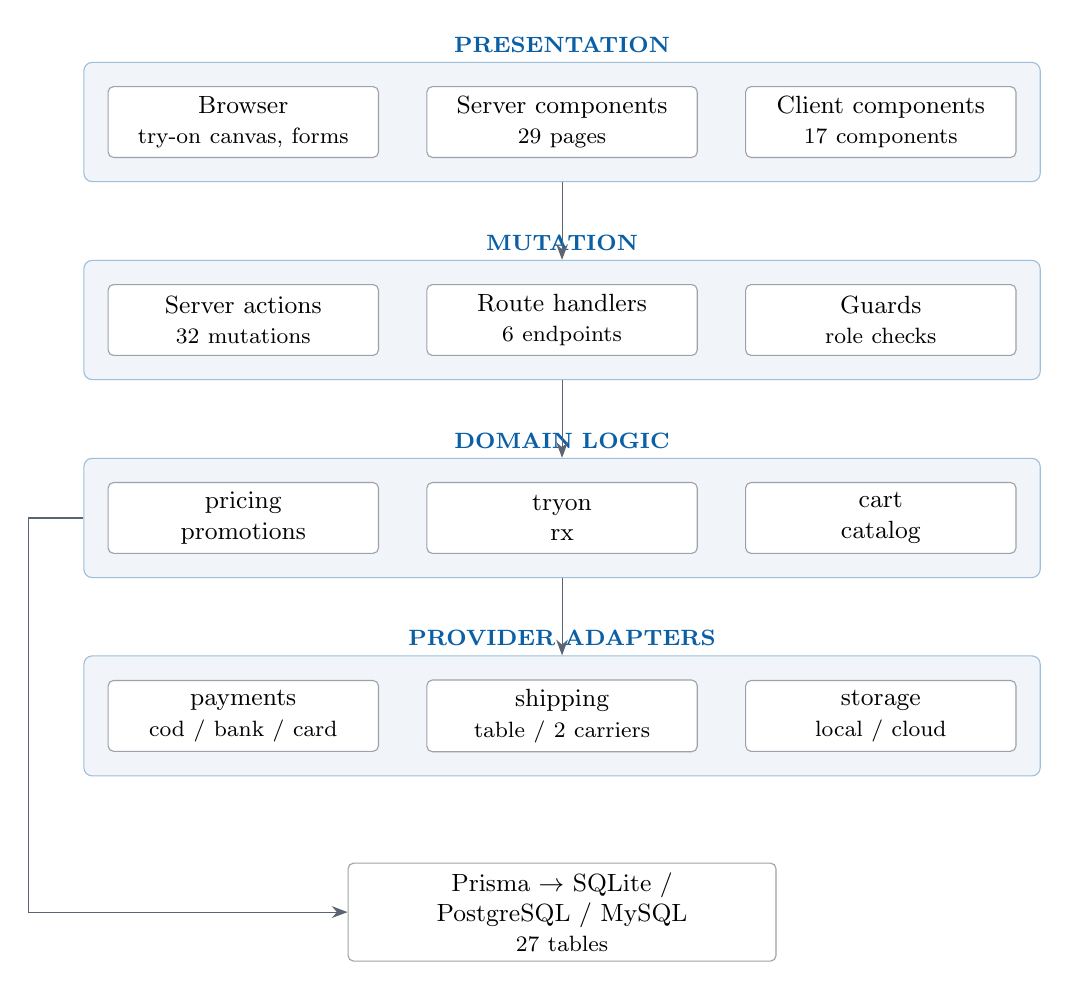
\begin{tikzpicture}[
  node distance=6mm,
  box/.style={draw=vcgrey!60,fill=white,rounded corners=2pt,minimum height=9mm,
              align=center,font=\small,text width=32mm},
  band/.style={draw=vcblue!40,fill=vclight,rounded corners=3pt,inner sep=3mm},
  lbl/.style={font=\footnotesize\bfseries\color{vcblue}},
  arr/.style={-{Stealth[length=2mm]},draw=vcgrey}
]

\node[box] (b1) {Browser\\\footnotesize try-on canvas, forms};
\node[box,right=of b1] (b2) {Server components\\\footnotesize 29 pages};
\node[box,right=of b2] (b3) {Client components\\\footnotesize 17 components};
\begin{scope}[on background layer]
  \node[band,fit=(b1)(b2)(b3),label={[lbl]above:PRESENTATION}] (P) {};
\end{scope}

\node[box,below=16mm of b1] (m1) {Server actions\\\footnotesize 32 mutations};
\node[box,right=of m1] (m2) {Route handlers\\\footnotesize 6 endpoints};
\node[box,right=of m2] (m3) {Guards\\\footnotesize role checks};
\begin{scope}[on background layer]
  \node[band,fit=(m1)(m2)(m3),label={[lbl]above:MUTATION}] (M) {};
\end{scope}

\node[box,below=16mm of m1] (d1) {pricing\\promotions};
\node[box,right=of d1] (d2) {tryon\\rx};
\node[box,right=of d2] (d3) {cart\\catalog};
\begin{scope}[on background layer]
  \node[band,fit=(d1)(d2)(d3),label={[lbl]above:DOMAIN LOGIC}] (D) {};
\end{scope}

\node[box,below=16mm of d1] (a1) {payments\\\footnotesize cod / bank / card};
\node[box,right=of a1] (a2) {shipping\\\footnotesize table / 2 carriers};
\node[box,right=of a2] (a3) {storage\\\footnotesize local / cloud};
\begin{scope}[on background layer]
  \node[band,fit=(a1)(a2)(a3),label={[lbl]above:PROVIDER ADAPTERS}] (A) {};
\end{scope}

\node[box,below=14mm of a2,text width=52mm] (db)
  {Prisma $\rightarrow$ SQLite / PostgreSQL / MySQL\\\footnotesize 27 tables};

\draw[arr] (P) -- (M);
\draw[arr] (M) -- (D);
\draw[arr] (D) -- (A);
\draw[arr] (D.west) -- ++(-7mm,0) |- (db.west);
\end{tikzpicture}
\caption{The five layers. Each one may call downwards, never upwards.}
\end{figure}

\section{Directory map}

\begin{lstlisting}
prisma/
  schema.prisma          27 models, portable across three databases
  seed.ts                staff, catalogue, lenses, rates, promotions, demo data
  migrations/            one migration, 19.8 KB of SQL

scripts/
  fetch-tryon-assets.mjs copies the WebAssembly runtime, downloads the model
  generate-frame-assets.mjs draws placeholder frame artwork

public/
  models/                face_landmarker.task   3.6 MB
  wasm/                  MediaPipe runtime      34 MB
  frames/                31 generated overlays  1.1 MB
  uploads/               locally stored images

src/
  app/
    (shop)/              13 storefront pages
    admin/               16 back-office pages
    actions/             32 server actions in 4 files
    api/                 6 route handlers
  components/
    tryon/               the virtual mirror (3 files, 854 lines)
    shop/                8 storefront components
    admin/               7 back-office components
  lib/                   17 modules -- the domain layer
\end{lstlisting}

\section{Size of the codebase}

\begin{center}
\begin{tabular}{@{}lr@{}}
\toprule
\textbf{Measure} & \textbf{Count}\\
\midrule
TypeScript and TSX source lines & 13{,}676\\
Schema, seed data and asset scripts & 1{,}618\\
Source files & 77\\
Database tables & 27\\
Storefront pages & 13\\
Back-office pages & 16\\
Web API endpoints & 6\\
Server actions & 32\\
React components & 17\\
Domain library modules & 17\\
Audit call sites & 26\\
Type errors & 0\\
Lint warnings & 0\\
\bottomrule
\end{tabular}
\end{center}

\chapter{The data model}

\section{The 27 tables, grouped}

\begin{longtable}{@{}p{0.20\textwidth}p{0.24\textwidth}p{0.48\textwidth}@{}}
\toprule
\textbf{Group} & \textbf{Tables} & \textbf{Purpose}\\
\midrule
\endhead
People and access &
\code{User}, \code{Patient}, \code{Prescription}, \code{PatientDocument},
\code{Appointment}, \code{Address} &
The clinical record. Every customer, whether registered or a guest, gets a
patient file with a sequential number such as \code{P-000042}.\\
\addlinespace
Catalogue &
\code{Brand}, \code{Category}, \code{FrameCategory}, \code{Frame},
\code{FrameVariant}, \code{ProductImage} &
A frame is a model; a variant is one colourway of it, carrying its own stock,
barcode, price override and try-on calibration.\\
\addlinespace
Lenses &
\code{LensOption} &
One table drives the entire six-step lens wizard, its prices, its
prescription limits and its compatibility rules.\\
\addlinespace
Commerce &
\code{Cart}, \code{CartItem}, \code{Order}, \code{OrderItem},
\code{Payment}, \code{Shipment}, \code{ShippingRate} &
Baskets, orders, money and parcels. Order lines carry frozen snapshots of
everything that mattered at the moment of sale.\\
\addlinespace
Marketing &
\code{Promotion} &
Six kinds of deal, each with nine possible conditions.\\
\addlinespace
Virtual try-on &
\code{TryOnSession}, \code{TryOnSnapshot} &
Only ever written when a signed-in customer explicitly saves a picture and the
shop has that feature enabled.\\
\addlinespace
Operations &
\code{Setting}, \code{MediaAsset}, \code{ImportJob}, \code{AuditLog} &
Shop configuration a manager can change without a developer; the image
library; spreadsheet job history; and the trail of who changed what.\\
\bottomrule
\end{longtable}

\section{The relationships that carry the design}

\begin{figure}[H]
\centering
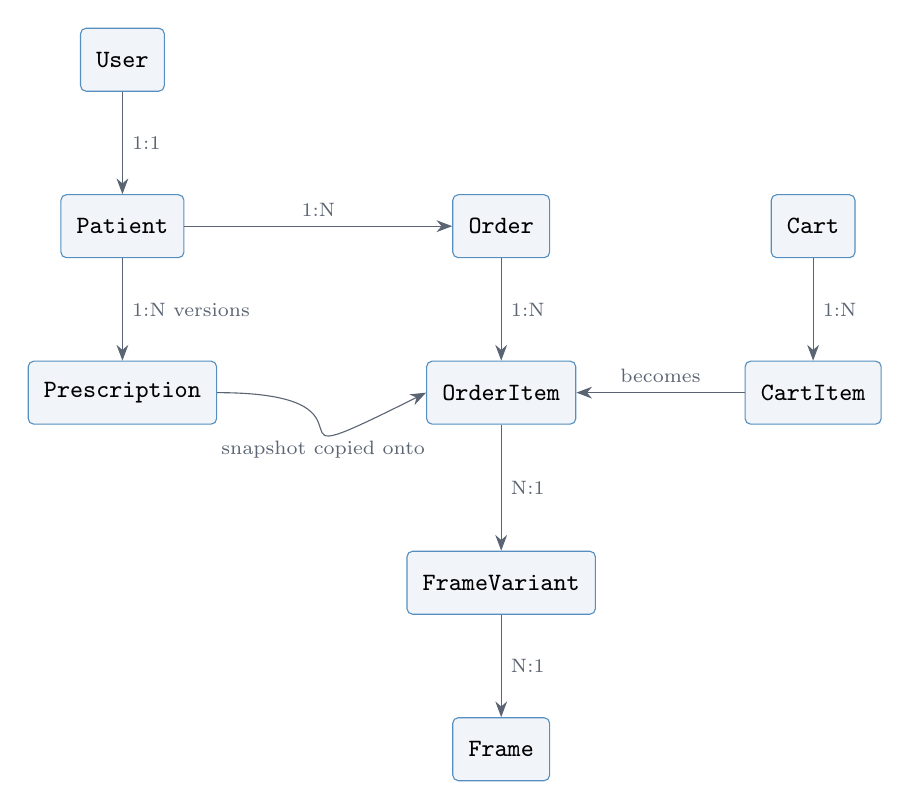
\begin{tikzpicture}[
  e/.style={draw=vcblue!70,fill=vclight,rounded corners=2pt,
            minimum height=8mm,font=\small\ttfamily,inner sep=2mm},
  r/.style={-{Stealth[length=2mm]},draw=vcgrey,font=\scriptsize\color{vcgrey}},
  node distance=13mm and 20mm
]
\node[e] (user) {User};
\node[e,below=of user] (patient) {Patient};
\node[e,below=of patient] (rx) {Prescription};
\node[e,right=34mm of patient] (order) {Order};
\node[e,below=of order] (oitem) {OrderItem};
\node[e,right=28mm of order] (cart) {Cart};
\node[e,below=of cart] (citem) {CartItem};
\node[e,below=16mm of oitem] (variant) {FrameVariant};
\node[e,below=of variant] (frame) {Frame};

\draw[r] (user) -- node[right]{1:1} (patient);
\draw[r] (patient) -- node[right]{1:N versions} (rx);
\draw[r] (patient) -- node[above]{1:N} (order);
\draw[r] (order) -- node[right]{1:N} (oitem);
\draw[r] (cart) -- node[right]{1:N} (citem);
\draw[r] (citem) -- node[above]{becomes} (oitem);
\draw[r] (oitem) -- node[right]{N:1} (variant);
\draw[r] (variant) -- node[right]{N:1} (frame);
\draw[r] (rx.east) .. controls +(2.4,0) and +(-2.4,-1.2) ..
      node[below,pos=0.55]{snapshot copied onto} (oitem.west);
\end{tikzpicture}
\caption{The spine of the model. Note the curved relationship: an order line
does not merely \emph{point at} a prescription, it also stores its own frozen
copy of it.}
\end{figure}

\section{Three invariants the schema enforces}

\begin{enumerate}
  \item \textbf{Everyone has a patient file.} Registration creates one
        automatically. So does a guest checkout --- matched on email address so
        a returning guest keeps the same file rather than accumulating new
        ones. An optical order that cannot be traced to a patient cannot be
        remade or followed up.

  \item \textbf{Prescriptions are versioned, never overwritten.} Statuses run
        \emph{draft}, \emph{pending verification}, \emph{verified},
        \emph{rejected}, \emph{expired}. A customer-entered prescription
        always begins as \emph{pending verification} and appears in the
        optician's queue. The lab ticket refuses to look ready until a
        qualified person has verified it.

  \item \textbf{Order lines are self-contained history.} Each line stores its
        own title, SKU, image, unit price, lens price, lens option codes, a
        lens summary and a complete frozen prescription including the pupil
        distance. An invoice from three years ago still reads correctly even
        if the product has since been renamed, re-priced or deleted.
\end{enumerate}

\chapter{How a request travels through the system}

\section{Reading a page}

\begin{enumerate}
  \item The browser asks for a web address, for example \code{/frames/ravi}.
  \item Next.js matches it to a server component, which runs on the server.
  \item That component calls a library module in \code{src/lib} ---
        \code{catalog.ts} for the product, \code{pricing.ts} for the price.
  \item The library module queries the database through Prisma.
  \item Finished HTML is streamed to the browser. Only the interactive parts
        --- the lens builder and the try-on canvas --- also send code.
\end{enumerate}

\section{Changing something}

\begin{enumerate}
  \item The user submits a form.
  \item The form calls a \emph{server action} directly. No hand-written web
        API sits in between.
  \item The action first runs its guard. Staff actions call \code{staff()};
        pages call \code{requireStaff()} or \code{requireAdmin()}. All 20
        back-office actions were verified to carry a guard.
  \item The action validates its input with Zod.
  \item It performs the change, wrapping multi-table work in a database
        transaction.
  \item It writes an audit entry.
  \item It tells Next.js which cached pages are now stale so the screen
        refreshes.
\end{enumerate}

\keybox{Why route handlers still exist}{Server actions cannot stream a large
file upload, cannot return a downloadable spreadsheet, and cannot receive a
signed webhook from a payment provider. Those three cases --- and only those
three --- use the six conventional web API endpoints under \code{src/app/api}.}

\section{Placing an order, in detail}

This is the most complex path in the system. It is worth following because
almost every design decision in the project shows up in it.

\begin{enumerate}
  \item The submitted form is validated against a schema.
  \item The chosen payment method is checked against the methods the shop has
        actually enabled --- a tampered form cannot select a disabled one.
  \item \textbf{The entire basket is re-priced from the database.} Nothing the
        browser sent about price is trusted.
  \item Out-of-stock lines block the order.
  \item If the shop requires a prescription on every pair, every line is
        checked for one.
  \item Discounts are re-evaluated from scratch.
  \item Delivery is re-quoted for the address actually entered.
  \item Totals are computed: goods, minus discount, plus delivery, plus tax.
  \item A patient file is found or created.
  \item A sequential order number is allocated, in the form
        \code{VC-2026-000001}.
  \item \textbf{Inside one database transaction:} the address is stored, the
        order is created, and for each line --- any prescription typed at
        checkout is promoted into a real versioned record marked \emph{pending
        verification}, the order line is written with its frozen snapshot, and
        stock is decremented.
  \item The basket is emptied but the row is kept for analytics.
  \item An audit entry is written.
  \item Payment is started. If the payment provider fails, the order is
        \emph{not} discarded --- it is marked payment-failed with a note, so
        staff can take payment by hand rather than lose the sale.
  \item A shipment record is created and the customer is sent either to the
        provider's payment page or to their order page.
\end{enumerate}

\chapter{The virtual try-on engine}

\section{The idea in one paragraph}

A frame overlay is a transparent picture plus two \emph{anchors}: the points
inside that picture where the wearer's pupils ought to sit. Given the
customer's two pupils in their photograph, there is \textbf{exactly one}
similarity transform --- a uniform scale, a rotation and a shift --- that puts
the anchors on the pupils. That single fact is the entire placement algorithm.
There is no per-face tuning, no machine learning at drawing time, and nothing
to go subtly wrong.

\section{The mathematics}

Let $a_L, a_R$ be the anchor points expressed in the overlay's own pixels, and
$p_L, p_R$ the customer's pupils in canvas pixels. Write $k$ for a per-artwork
correction factor and $s_u, \theta_u, \Delta_u$ for the customer's own manual
nudges.

\begin{align}
\text{scale} \quad s &= \frac{\lVert p_R - p_L \rVert}{\lVert a_R - a_L \rVert}\cdot k \cdot s_u \\[4pt]
\text{rotation} \quad \theta &=
  \operatorname{atan2}\!\left(p_{R_y}-p_{L_y},\; p_{R_x}-p_{L_x}\right)
  -\operatorname{atan2}\!\left(a_{R_y}-a_{L_y},\; a_{R_x}-a_{L_x}\right)
  +\theta_u \\[4pt]
\text{translation} \quad t &= p_L + \Delta_u
\end{align}

The overlay is then drawn by translating to $t$, rotating by $\theta$, scaling
by $s$, and translating back by $-a_L$.

\section{Measuring pupil distance without a ruler}

Pupil distance --- the separation between the centres of the two pupils --- is
essential for making lenses and almost nobody knows their own. The trick used
here is that the visible iris of an adult eye is 11.7\,mm across and varies
remarkably little between people. It therefore works as a ruler that is
already in the photograph.

\begin{equation}
\text{PD}_{\text{mm}} \;=\;
\lVert p_R - p_L \rVert_{\text{px}} \times
\frac{11.7}{\bar{d}_{\text{iris,px}}}
\end{equation}

where $\bar{d}_{\text{iris,px}}$ is the mean of the two measured iris widths.
Expect roughly $\pm 2$\,mm.

\subsection{Knowing when not to trust the number}

The system reports a confidence score rather than a bare figure:

\begin{equation}
c \;=\; \operatorname{clamp}_{[0,1]}\!\left(
1 - 2.5\,\alpha - 0.5\min\!\left(1, \tfrac{|\rho|}{25}\right)\right),
\qquad
\alpha = \frac{\bigl|d_L - d_R\bigr|}{\max(d_L, d_R)}
\end{equation}

Here $\alpha$ is the asymmetry between the two measured irises and $\rho$ is
the head roll in degrees. Irises of visibly different width mean the head is
turned away from the camera, which breaks the assumption that both pupils lie
in one plane. A prescription of implausible width --- below 48\,mm or above
80\,mm --- has its confidence capped at 0.2 rather than being reported as
fact.

\keybox{An honest measurement}{The number is only written to the patient's
file when confidence reaches 0.5 \emph{and} no optician has already recorded a
pupil distance by hand. A machine estimate never overwrites a human
measurement. The customer is always told an optician will confirm it.}

\section{Graceful degradation}

If the browser is too old, the model file is missing, or the photograph simply
defeats detection, the studio does not fail. It reports the detector as
unavailable and lets the customer drag two markers onto their own eyes.
Everything downstream --- placement, measurement, saving --- is then
identical. The feature degrades; it never breaks.

\section{The calibration workflow}

Adding artwork for a real frame is a back-office task:

\begin{enumerate}
  \item Open the frame, then a colourway, then the virtual-try-on tab.
  \item Upload a front-on transparent picture with the temples pointing out.
  \item Drag the \textbf{L} and \textbf{R} markers onto the centre of each
        lens.
  \item Check the live preview against a reference face and save.
\end{enumerate}

Colourways without artwork simply do not appear in the mirror, and the frame
page warns staff which ones are missing. The placeholder artwork shipped with
the project is drawn by a script so that a fresh installation has a working
shop before any photography has been done.

\keybox{A coupling worth knowing about}{The default anchor positions live in
\code{src/lib/tryon.ts} and the matching geometry constants live in
\code{scripts/generate-frame-assets.mjs}. They are two halves of one contract.
Changing one without the other will misplace every generated frame.}

\chapter{Money, pricing and discounts}

\section{The integer rule}

\keybox{Money is never a decimal number in this system}{Every monetary value
is stored and calculated as a whole number of the smallest unit --- paisa, or
cents. Rs.\,6{,}500.00 is stored as the integer 650000. Staff type ordinary
amounts into forms and the conversion happens exactly once, at the edge.
Decimal arithmetic on money is how a shop ends up charging Rs.\,0.01 less than
it should on thousands of orders.}

There is one further subtlety: the display formatter deliberately avoids the
browser's built-in currency formatting, because that inserts a space whose
width differs between server and browser and causes the page to flicker on
load.

\section{One place decides the price}

Every price in the application is computed by \code{src/lib/pricing.ts}. No
component computes a total. The basket is re-priced from the database on
\emph{every single read}, which produces two useful properties:

\begin{itemize}
  \item A tampered payload from the browser cannot change what is charged.
  \item A price change or a stock change is reflected the instant the customer
        looks at their bag, with no cache to invalidate.
\end{itemize}

The same module also rejects lens combinations the laboratory cannot make ---
options that require each other, options that exclude each other, and options
whose prescription limits the customer's own prescription exceeds. Problems
are returned as readable sentences rather than thrown as errors, so the
interface can show them beside the choice that caused them.

\section{The discount engine}

Six kinds of deal are supported: percentage off, fixed amount off, free
delivery, buy-one-get-one, free lens upgrade, and bundle price. Each can be
restricted by nine conditions: minimum spend, minimum quantity, brand,
collection, specific frames, a date window, a total usage cap, a per-customer
cap, and first-orders-only.

\keybox{The stacking rule}{The highest-priority offer always applies. Any
other offer joins it only if \emph{every} promotion currently in play is
marked stackable. The effect is that a headline deal never silently doubles
up, but a delivery perk can ride alongside a discount code.}

Two details are worth noting. The buy-one-get-one calculation expands the
basket into individual units, sorts them by price and makes every second one
free from the cheapest end --- so the customer always keeps the more expensive
item. And when a customer types a code that does not apply, the engine
explains \emph{why} in words they can act on: expired, does not apply to
anything in the bag, needs more items, first orders only, or already used.

\chapter{Provider adapters}

Three parts of the system talk to the outside world. All three are built the
same way: one interface, several implementations, chosen by an environment
setting, each degrading safely when its key is absent.

\begin{longtable}{@{}p{0.16\textwidth}p{0.20\textwidth}p{0.56\textwidth}@{}}
\toprule
\textbf{Concern} & \textbf{Options} & \textbf{Behaviour}\\
\midrule
\endhead
Payments &
cash on delivery, bank transfer, card &
Cash and bank transfer need no account and work immediately. The card option
uses a hosted payment page, so card details never touch this server. Crucially
the order is confirmed by the provider's \emph{webhook}, not by the customer's
browser returning --- so a customer who closes the tab after paying still gets
their glasses. The card option hides itself entirely if no key is
configured.\\
\addlinespace
Shipping &
rate table, two live carriers &
The rate table is the default and needs no account. The two live options fetch
real carrier rates and can buy a real printable label. Both fall back to the
rate table if the key is missing or the call fails, so a carrier outage
degrades to flat-rate delivery instead of blocking checkout.\\
\addlinespace
Image storage &
local disk, cloud &
Local writes into the project's own public folder with zero setup. The cloud
option covers the three common providers and loads its library only when
actually used, so the dependency is not required unless it is wanted.\\
\bottomrule
\end{longtable}

Adding a fourth payment provider means writing one adapter function and adding
one entry to a list. Nothing about any provider leaks into the checkout
interface.

\chapter{Security, privacy and the audit trail}

\section{Sessions and passwords}

Sessions are signed tokens stored in a cookie that JavaScript cannot read, set
to expire after 30 days, and marked secure in production. Passwords are hashed
with bcrypt at 10 rounds. The sign-in form returns the \emph{same} message for
``no such account'' and ``wrong password'', so it cannot be used to discover
which email addresses have accounts. The application refuses to start if the
signing secret is missing or shorter than 32 characters.

\section{Four roles}

\begin{center}
\begin{tabular}{@{}lp{0.62\textwidth}@{}}
\toprule
\textbf{Role} & \textbf{Access}\\
\midrule
\code{customer} & The shop and their own account only.\\
\code{staff} & The back office.\\
\code{optician} & The back office, including prescription verification.\\
\code{admin} & Everything, including administrator-only screens.\\
\bottomrule
\end{tabular}
\end{center}

Guards are applied per page and per action rather than through a single global
filter. This was verified by request: the back office, the account area and
the checkout all redirect an unauthenticated visitor to the sign-in page.

\section{The audit trail}

Every change to a patient record, a price or an order writes a row recording
the actor, the action, the entity, the time and the client address. Even
spreadsheet exports of patient data are audited, because exporting clinical
data is itself an event worth recording.

\keybox{A deliberate omission}{Clinical values are kept \emph{out} of the audit
detail. The reasoning is that an audit log is read far more widely than the
record it describes, so putting prescriptions in it would quietly widen access
to health data. An audit failure also never takes down the operation it was
recording --- the write is wrapped so a logging problem cannot lose a sale.}

\section{Patient data provisions already in place}

The \code{Patient} table already carries a marketing-consent flag, the date
and version of consent given, a retention deadline and a soft-delete marker.
The data model is therefore ready for a retention policy; the policy decisions
themselves have not been made.

\section{What is still required before going live}

\begin{itemize}
  \item Encryption of the database at rest.
  \item A documented retention period, using the fields already present.
  \item A customer-facing route for correction and erasure requests.
  \item Rate limiting on sign-in and uploads (see the gaps chapter).
  \item Replacement of the seeded demonstration passwords.
\end{itemize}

% =========================================================================
\part{Running and operating the system}
% =========================================================================

\chapter{Installing and starting it}

\section{First run}

\begin{lstlisting}
npm install
cp .env.example .env
\end{lstlisting}

Open \code{.env} and set \code{AUTH\_SECRET} to a long random string. One can
be generated with:

\begin{lstlisting}
node -e "console.log(require('crypto').randomBytes(32).toString('hex'))"
\end{lstlisting}

Then build the database, fetch the face model, draw the placeholder artwork
and load the demonstration data:

\begin{lstlisting}
npm run setup
npm run dev
\end{lstlisting}

The shop appears at \code{http://localhost:3000} and the back office at
\code{http://localhost:3000/admin}.

\keybox{A note from this session}{On the machine used for this assessment port
3000 was already occupied by another program, so the development server was
started on an alternative port instead. This is normal and harmless. If it
happens, the address the server prints on startup is the one to use.}

\section{The demonstration accounts}

The seed data creates three accounts. Their passwords are published in the
project's own documentation, which means they are effectively public.

\begin{center}
\begin{tabular}{@{}lll@{}}
\toprule
\textbf{Role} & \textbf{Email} & \textbf{Password}\\
\midrule
Owner & \code{admin@visioncart.local} & \code{ChangeMe123!}\\
Optician & \code{optician@visioncart.local} & \code{Optician123!}\\
Customer & \code{demo@example.com} & \code{Demo1234!}\\
\bottomrule
\end{tabular}
\end{center}

\keybox{Change these before the shop is reachable from the internet}{Set the
seeded administrator email and password in \code{.env} before seeding, or
change the password from the back office afterwards. Leaving them in place on
a public server would hand anybody full access to every patient record.}

\section{Commands}

\begin{center}
\begin{tabular}{@{}ll@{}}
\toprule
\textbf{Command} & \textbf{What it does}\\
\midrule
\code{npm run dev} & Development server\\
\code{npm run build} & Production build\\
\code{npm run setup} & Migrate, fetch assets, draw artwork, seed\\
\code{npm run db:migrate} & Create and apply a database migration\\
\code{npm run db:seed} & Reload demonstration data (safe to repeat)\\
\code{npm run db:studio} & Browse the database in a window\\
\code{npm run db:reset} & Drop and rebuild the database\\
\code{npm run tryon:assets} & Re-fetch the face model and runtime\\
\code{npm run frames:generate} & Redraw the placeholder frame artwork\\
\code{npm run typecheck} & Check types across the whole project\\
\code{npm run lint} & Run the code linter\\
\bottomrule
\end{tabular}
\end{center}

\section{Configuration}

Only two settings are required to start: the database location and the signing
secret. Every integration degrades to a safe offline behaviour until real keys
are supplied, which is why the whole shop can be demonstrated before signing
up for anything.

Configuration is split deliberately. \textbf{Secrets and infrastructure} live
in the environment file and require a developer. \textbf{Anything a shop
manager should own} --- store details, free-delivery threshold, return window,
guest checkout, whether a prescription is compulsory, and the three try-on
switches --- lives in the database and is editable from the settings screen.

\chapter{Moving to production}

\begin{enumerate}
  \item \textbf{Switch to PostgreSQL.} Change the provider in the schema,
        point the database address at the new server and deploy the migration.
        Because the schema avoids enumerations, arrays and native JSON, no
        other edit is needed.
  \item \textbf{Replace every secret.} A fresh signing secret, new staff
        passwords, real payment keys.
  \item \textbf{Set the public address correctly}, because the payment
        provider's return links are built from it.
  \item \textbf{Move image storage to the cloud} unless the server has
        durable, backed-up disk.
  \item \textbf{Point the payment webhook} at the project's webhook endpoint
        and set its signing secret.
  \item \textbf{Set the tax rate}, expressed in basis points, and say whether
        displayed prices already include it.
  \item \textbf{Complete the four compulsory gaps} listed in the completion
        chapter: email, the guide pages, password recovery and rate limiting.
\end{enumerate}

% =========================================================================
\appendix
% =========================================================================

\chapter{Route reference}

\section{Storefront}

\begin{center}
\begin{tabular}{@{}ll@{}}
\toprule
\textbf{Address} & \textbf{Page}\\
\midrule
\code{/} & Home\\
\code{/frames} & Catalogue with filters\\
\code{/frames/[slug]} & Product page and lens builder\\
\code{/try-on} & Virtual mirror\\
\code{/deals} & Current offers\\
\code{/cart} & Shopping bag\\
\code{/checkout} & Checkout\\
\code{/order/[orderNo]} & Order confirmation and tracking\\
\code{/login}, \code{/register} & Access\\
\code{/account} & Customer account\\
\code{/account/orders} & Order history\\
\code{/account/prescriptions} & Saved prescriptions\\
\bottomrule
\end{tabular}
\end{center}

\section{Back office}

\begin{center}
\begin{tabular}{@{}ll@{}}
\toprule
\textbf{Address} & \textbf{Screen}\\
\midrule
\code{/admin} & Dashboard\\
\code{/admin/orders}, \code{/admin/orders/[id]} & Orders and lab tickets\\
\code{/admin/patients}, \code{/admin/patients/[id]} & Patient files\\
\code{/admin/patients/new} & New patient\\
\code{/admin/frames}, \code{/admin/frames/[id]} & Catalogue\\
\code{/admin/frames/new} & New frame\\
\code{/admin/media} & Image library\\
\code{/admin/lenses} & Lens options and prices\\
\code{/admin/promotions}, \code{/admin/promotions/[id]} & Deals\\
\code{/admin/promotions/new} & New deal\\
\code{/admin/import} & Spreadsheet import and export\\
\code{/admin/settings} & Store settings\\
\bottomrule
\end{tabular}
\end{center}

\section{Web API endpoints}

\begin{center}
\begin{tabular}{@{}ll@{}}
\toprule
\textbf{Endpoint} & \textbf{Why it is not a server action}\\
\midrule
\code{/api/admin/upload} & Streams a multipart file upload\\
\code{/api/admin/import} & Streams a spreadsheet upload\\
\code{/api/admin/export} & Returns a downloadable file\\
\code{/api/account/prescription-upload} & Streams a file upload\\
\code{/api/tryon/snapshot} & Streams an image upload\\
\code{/api/webhooks/stripe} & Receives a signed external callback\\
\bottomrule
\end{tabular}
\end{center}

\section{Known broken links}

\begin{center}
\begin{tabular}{@{}ll@{}}
\toprule
\textbf{Address linked from every page footer} & \textbf{Result}\\
\midrule
\code{/guides/prescription} & 404 not found\\
\code{/guides/pd} & 404 not found\\
\code{/guides/returns} & 404 not found\\
\code{/guides/privacy} & 404 not found\\
\bottomrule
\end{tabular}
\end{center}

\chapter{The domain library}

The seventeen modules in \code{src/lib} are where the actual thinking lives.

\begin{longtable}{@{}p{0.22\textwidth}r p{0.56\textwidth}@{}}
\toprule
\textbf{Module} & \textbf{Lines} & \textbf{Responsibility}\\
\midrule
\endhead
\code{tryon.ts} & 303 & Placement geometry and pupil-distance measurement.
Pure functions, no browser and no server imports, so the same mathematics runs
in the canvas, in a test and on the server.\\
\code{shipping.ts} & 324 & Three delivery providers behind one interface.\\
\code{payments.ts} & 291 & Three payment providers behind one interface.\\
\code{promotions.ts} & 261 & Deal evaluation, eligibility and stacking.\\
\code{pricing.ts} & 221 & The only place a price is decided.\\
\code{constants.ts} & 217 & Every permitted value in the system.\\
\code{cart.ts} & 215 & Basket identity, merging a guest bag on sign-in.\\
\code{catalog.ts} & 206 & Shared catalogue queries and filters.\\
\code{storage.ts} & 197 & Image processing and two storage back-ends.\\
\code{rx.ts} & 181 & Prescription validation and clinical helpers.\\
\code{auth.ts} & 147 & Sign-in, registration, patient files, guards.\\
\code{csv.ts} & 102 & Spreadsheet parsing and writing, from scratch.\\
\code{session.ts} & 75 & Signed session cookies.\\
\code{settings.ts} & 53 & Shop configuration with defaults.\\
\code{money.ts} & 49 & Integer money and display formatting.\\
\code{audit.ts} & 39 & The audit trail.\\
\code{db.ts} & 14 & The database connection, cached across reloads.\\
\bottomrule
\end{longtable}

\chapter{Glossary for the non-technical reader}

\begin{longtable}{@{}p{0.24\textwidth}p{0.70\textwidth}@{}}
\toprule
\textbf{Term} & \textbf{Meaning}\\
\midrule
\endhead
Anchor & The two points marked inside a frame picture showing where the
wearer's pupils should sit. Calibrating a frame means placing these two
points.\\
\addlinespace
Axis & The angle, from 1 to 180 degrees, at which an astigmatism correction
is oriented. Meaningless without a cylinder value.\\
\addlinespace
Colourway or variant & One colour of one frame model. Stock, barcode, price
and try-on calibration all belong to the colourway, not the model.\\
\addlinespace
Cylinder & The strength of the astigmatism correction, in the same 0.25 steps
as the sphere.\\
\addlinespace
Diopter & The unit of lens strength. Written with a sign and two decimals,
always in steps of 0.25.\\
\addlinespace
Migration & A recorded change to the shape of the database, so the same change
can be applied to another copy in the same order.\\
\addlinespace
Minor units & The smallest denomination of a currency: paisa, cents. All money
in this system is stored as a whole number of these.\\
\addlinespace
OD and OS & Latin abbreviations for the right eye and the left eye, used on
every prescription in the world.\\
\addlinespace
PD, pupillary distance & The distance in millimetres between the centres of
the two pupils. Needed to position the optical centre of each lens.\\
\addlinespace
Seeding & Loading a set of realistic starting data so a fresh installation has
a working shop to look at.\\
\addlinespace
Server action & A function that a form can call directly, which runs on the
server. Used here instead of building a separate web API.\\
\addlinespace
Sphere & The main strength of a lens. Negative for short sight, positive for
long sight.\\
\addlinespace
WebAssembly & A format that lets demanding code, such as face detection, run
at near-native speed inside a web browser.\\
\bottomrule
\end{longtable}

\chapter{Summary card}

\keybox{VisionCart at a glance}{
\textbf{What it is:} a complete online opticians' shop with an in-browser
virtual try-on and a full clinical back office.\\[4pt]
\textbf{Built with:} Next.js 16, React 19, TypeScript, Tailwind 4, Prisma and
MediaPipe.\\[4pt]
\textbf{Size:} 13{,}676 lines of source across 77 files, 27 database tables,
29 pages, 32 server actions.\\[4pt]
\textbf{Health:} zero type errors, zero lint warnings, runs correctly.\\[4pt]
\textbf{Completion:} roughly 85\% as a product, about 70\% ready for the
public.\\[4pt]
\textbf{Blocking work before launch:} transactional email, four missing guide
pages, password recovery, rate limiting.\\[4pt]
\textbf{Strongest parts:} the try-on geometry, the clinical data rules, the
single-source pricing engine, and the provider adapters.\\[4pt]
\textbf{Weakest parts:} no tests, no notifications, no audit viewer.}

\vfill
\begin{center}
\color{vcgrey}\small
This manual was produced by inspecting the running application and every
source file in the project. Percentages are informed judgements; every
specific claim about behaviour was verified either in the browser or in the
source.
\end{center}

\end{document}
